\documentclass[10pt]{beamer}
\usepackage{graphicx}
\usepackage{listings}
\usepackage{multicol}
\usepackage{tikz}
\usetikzlibrary{calc}
%\usepackage{showframe}

\mode<presentation>{
    \usetheme{redhat}
%    \setbeameroption{show notes on second screen=bottom}
}

% https://github.com/josephwright/beamer/issues/337
%\makeatletter
%\def\beamer@framenotesbegin{%
%    \usebeamercolor[fg]{normal text}%
%    \gdef\beamer@noteitems{}%
%    \gdef\beamer@notes{}%
%}
%\makeatother

\setcounter{tocdepth}{1}
\newcommand{\autotitle}{
    \frametitle{
        \secname
        \ifx \insertsubsection \empty \else { / \MakeLowercase{\subsecname}} \fi
    }
}

\newcommand{\sectiontitleframe}{
    \vspace{-1em} % XXX
    \begin{beamercolorbox}[wd=\paperwidth]{title page}
        \begin{tikzpicture}[text = white]
            \fill[above left, color=redhat]
                (0, 2em)
                rectangle (\the\paperwidth, \the\paperheight);
            \node (title)
                [xshift = -2em, yshift = 2em, text width = 0.75\textwidth]
                at (current page.center)
                {\Large\bfseries\secname};
        \end{tikzpicture}
    \end{beamercolorbox}
}

\title{End-to-End Tests in OpenShift}

\author{Bruno Barcarol Guimarães}
\institute[]{Red Hat}
\date{2022-07-14}

\begin{document}

\begin{frame}
    \titlepage
\end{frame}

\begin{frame}
    \frametitle{Overview}
    \tableofcontents
\end{frame}

\section{Introduction}
\begin{frame}
    \autotitle
    \begin{itemize}
        \item \url{https://docs.google.com/document/d/1md-1BMf4_7mtKgGVoeZ3jOh4zSIBSjwl6vTTAYESwIM}
            \begin{itemize}
                \item
                    \normalsize
                    \textit{Multi-Stage Tests Design Document}
            \end{itemize}
        \item \url{https://docs.ci.openshift.org}
            \begin{itemize}
                \item \href
                    {https://docs.ci.openshift.org/docs/architecture/step-registry/}
                    {\texttt{docs/architecture/step-registry}}
                \item \href
                    {https://docs.ci.openshift.org/docs/architecture/ci-operator/}
                    {\texttt{docs/architecture/ci-operator}}
            \end{itemize}
    \end{itemize}
    \note{
        Documentation for the topics covered today is somewhat scattered among
        several pages.  The main content is in the dedicated step registry page,
        but some descriptions and examples can also be found in more general
        pages such as \texttt{ci-operator} and others.

        The original design document is also a good source of information about
        the basic architecture.  It also describes very well the historical
        context in which multi-stage tests and the step registry were developed
        and added to \texttt{ci-operator} and the OpenShift CI.
    }
\end{frame}

\subsection{Motivation}

\begin{frame}
    \autotitle
    ca. Aug 2019
    \begin{itemize}
        \item Two test types.
            \begin{itemize}
                \item container
                \item template
            \end{itemize}
        \item Desire to create tests for increasingly varied scenarios.
        \item Existing tests already complex and barely maintained.
    \end{itemize}
    \note{
        That context in summary is this: \texttt{ci-operator} started its life
        supporting only simple \textit{container} tests.  These are fairly
        self-contained tests which execute a single command using a container
        image.

        Then (likely on a Sunday), \textit{template} tests were added.  These
        were amorphous tests which bypassed most of the configuration format and
        instead injected a new test definition at runtime.  Creating and
        maintaining a template test was unnecessarily difficult, so practically
        only a few people had the knowledge and the stomach to do it.

        At the same time, the OpenShift CI was growing, being used both by more
        components and for more varied types of tests.  It was clear that
        requiring a new template test for each new test scenario would be
        impossible, so a new format for test definitions had to be created.
    }
\end{frame}

\begin{frame}
    \autotitle
    Ah, the templates\ldots
    \vfill
    \begin{quote}
complex, esoteric and fragile
    \end{quote}
    \vfill
    \begin{quote}
difficult to extend and use
    \end{quote}
    \vfill
    \begin{quote}
not able to share common test logic
    \end{quote}
    \vfill
    \begin{quote}
duplication and fragmentation
    \end{quote}
    \vfill
    \note{
        This sentiment is visible in the design document, which constantly
        mentions the limitations of templates which impeded the maintenance of
        existing and creation of new tests.
    }
\end{frame}

\begin{frame}
    \autotitle
    \begin{itemize}
        \item Small number of extremely complex \texttt{Pod} definitions.
            \begin{itemize}
                \item
                    Python embedded in Bash embedded in YAML embedded in
                    \ldots
                \item Each responsible for the entire execution of an E2E test.
            \end{itemize}
        \item
            Equally small set of people willing to / capable of ``maintaining''
            them.
        \item Adding a new test scenario
            \begin{itemize}
                \item copying an existing template (thousands of lines of YAML)
                \item minor edits
                \item (extreme duplication)
            \end{itemize}
        \item
            Configuration exposed and required knowledge of byzantine
            implementation details of \texttt{ci-operator}.
        \item<2> \emph{etc.}
    \end{itemize}
    \note{
        Here is a small selection (an entire presentation could be made about
        them):

        \begin{itemize}
            \item
                Template tests are defined in a single YAML file containing,
                among other items, a \texttt{Pod} definition.  The definition
                consisted of several inline \texttt{bash} scripts, sometimes
                with multiple fragments of other languages inside them.
            \item
                The entirety of the test flow had to be contained in this single
                YAML file.
            \item
                Because definitions were completely self-contained, creating new
                types of tests required blindly copying colossal YAML files and
                editing usually just a few lines, creating massive duplication
                and divergence.  Changing common code required editing all
                copies.
            \item
                The integration with other parts of \texttt{ci-operator}
                (images, releases, etc.) was very precarious, requiring test
                authors to know obscure aspects of the underlying
                implementation.
        \end{itemize}

        For these reasons and many others, the set of maintainers of these test
        definitions was virtually non-existent.
    }
\end{frame}

\section{Test types}
\begin{frame}
    \sectiontitleframe
    \note{(we have fancy section title slides now)}
\end{frame}

\begin{frame}[fragile]
    \autotitle
    \href
        {https://github.com/openshift/release/blob/master/ci-operator/config/openshift/origin/openshift-origin-master.yaml}
        {ibid}
    \begin{verbatim}
- as: verify-deps
  commands: make verify-deps …
  container:
    from: src
    \end{verbatim}
    \href
        {https://github.com/openshift/release/blob/master/ci-operator/config/openshift/origin/openshift-origin-release-3.11.yaml}
        {\ttfamily\ldots/openshift-origin-release-3.11.yaml}
    \begin{verbatim}
- as: e2e-gcp
  commands: … run-tests
  openshift_ansible:
    cluster_profile: gcp
    \end{verbatim}
    \note{
        The \texttt{test} entries in the configuration file have many different
        forms, although they have many similarities.  \texttt{steps} (or,
        sometimes, \texttt{literal\_steps}, as in the previous example), denotes
        a \textit{multi-stage} test.  Other basic test types are:
        \begin{itemize}
            \item
                simple \textit{container} tests, declared with
                \texttt{container}
            \item
                a large variety of \textit{template} tests, declared with fields
                in the form \texttt{openshift\_*}
        \end{itemize}
    }
\end{frame}

\begin{frame}[fragile]
    \autotitle
    \url{https://github.com/openshift/ci-tools/blob/master/pkg/api/types.go}
    \vfill
    \footnotesize
    \begin{verbatim}
type TestStepConfiguration struct {
    As string ` json:"as"`
    Commands string ` json:"commands,omitempty"`
    // …
    // Only one of the following can be not-null.
    ContainerTestConfiguration                                …
    MultiStageTestConfiguration                               …
    MultiStageTestConfigurationLiteral                        …
    OpenshiftAnsibleClusterTestConfiguration                  …
    OpenshiftAnsibleSrcClusterTestConfiguration               …
    OpenshiftAnsibleCustomClusterTestConfiguration            …
    OpenshiftInstallerClusterTestConfiguration                …
    OpenshiftInstallerUPIClusterTestConfiguration             …
    OpenshiftInstallerUPISrcClusterTestConfiguration          …
    OpenshiftInstallerCustomTestImageClusterTestConfiguration …
}
    \end{verbatim}
    \vfill
    \note{
        This is manifested in code in the \texttt{TestStepConfiguration}
        structure (not to be confused with the \texttt{TestStep} structure, used
        in multi-stage tests), which uses the common pattern of many (optional)
        pointers to other structures, only one of which is ever non-null (a
        \textit{sum type}).
    }
\end{frame}

\subsection{Container}

\begin{frame}[fragile]
    \autotitle
    \begin{verbatim}
// Only one of the following can be not-null.
ContainerTestConfiguration \
    *ContainerTestConfiguration \
    ` json:"container,omitempty"`
// …
    \end{verbatim}
    \note{
        (these identifiers are enormous, so here is what a full line looks like)
    }
\end{frame}

\begin{frame}[fragile]
    \autotitle
    \begin{verbatim}
type ContainerTestConfiguration struct {
    From PipelineImageStreamTagReference
    MemoryBackedVolume *MemoryBackedVolume
    Clone *bool
}
    \end{verbatim}
    \note{
        Starting with container tests, their structure is deceptively simple.
        It declares its container image plus a couple of other, more esoteric
        fields.
    }
\end{frame}

\begin{frame}[fragile]
    \autotitle
    \begin{verbatim}
type TestStepConfiguration struct {
    As string
    Commands string
    Cluster Cluster
    Secret *Secret
    Secrets []*Secret
    Cron *string
    Interval *string
    ReleaseController bool
    Postsubmit bool
    ClusterClaim *ClusterClaim
    RunIfChanged string
    Optional bool
    SkipIfOnlyChanged string
    Timeout *prowv1.Duration
    // …
    \end{verbatim}
    \note{
        This is because most of the fields live in the original structure,
        previously abbreviated.  The list of fields here is somewhat unruly.  In
        the past, we had a very relaxed policy for external contributions, so
        the code base --- and this area in particular --- grew very
        ``organically'' (to put it favorably).

        Some of these, such as the build cluster, the periodic/post-submit
        fields, etc. are still useful.  Some are obsolete and kept for
        compatibility.

        As an aside, the capabilities of container tests are roughly a subset of
        those of multi-stage, there is a long-term plan to unify their
        underlying implementation.
    }
\end{frame}

\subsection{Template}

\begin{frame}[fragile]
    \autotitle
    \begin{verbatim}
- as: e2e-gcp
  commands: … run-tests
  openshift_ansible:
    cluster_profile: gcp
    \end{verbatim}
    \footnotesize
    \begin{verbatim}
args:
- --image-import-pull-secret=/etc/pull-secret/.dockerconfigjson
- --report-credentials-file=/etc/report/credentials
- --secret-dir=/usr/local/e2e-gcp-periodic-cluster-profile
- --target=e2e-gcp-periodic
- --template=/usr/local/e2e-gcp-periodic
- --gcs-upload-secret=/secrets/gcs/service-account.json
command:
- ci-operator
    \end{verbatim}
    \note{
        The second type of test (also in chronological order) is everyone's
        favorite: template tests.  This was the first mechanism added to
        \texttt{ci-operator} to support end-to-end tests, or in general anything
        more complex than a container test.

        They are mostly a historical curiosity at this point, used only in very
        old, 3.11 jobs, but they provide some context to some of the more
        dubious aspects of \texttt{ci-operator}.

        There is no (with one exception due to a failed plan) corresponding test
        definition in the configuration file for these tests: the entry in
        \texttt{tests} is used exclusively by \texttt{prowgen}.  Instead, the
        definition is supplied at runtime via the \texttt{--template} argument.
    }
\end{frame}

\begin{frame}[fragile]
    \autotitle
    \begin{verbatim}
      volumeMounts:
      - mountPath: /usr/local/e2e-gcp-periodic
        name: job-definition
        subPath: cluster-launch-e2e.yaml
    volumes:
    - configMap:
        name: prow-job-cluster-launch-e2e
      name: job-definition
    \end{verbatim}
    \note{
        In our Prow jobs, this is done by mounting the definition via a
        \texttt{ConfigMap}\ldots
    }
\end{frame}

\begin{frame}[fragile]
    \autotitle
    \url{https://github.com/openshift/release/tree/master/ci-operator/templates}
    \vfill
    \footnotesize
    \begin{verbatim}
ci-operator/templates/
    master-sidecar-3.yaml
    master-sidecar-4.4.yaml
    openshift/
        installer/
            cluster-launch-installer-custom-test-image.yaml
            cluster-launch-installer-e2e.yaml
            cluster-launch-installer-libvirt-e2e.yaml
            cluster-launch-installer-metal-e2e.yaml
            cluster-launch-installer-openstack-e2e.yaml
            cluster-launch-installer-openstack-upi-e2e.yaml
            cluster-launch-installer-src.yaml
            cluster-launch-installer-upi-e2e.yaml
        openshift-ansible/
            cluster-launch-e2e-openshift-ansible.yaml
            cluster-launch-e2e.yaml
            cluster-scaleup-e2e-40.yaml
    \end{verbatim}
    \vfill
    \note{
        \ldots which in turn are populated via \texttt{updateconfig} from the
        files in the dreaded \texttt{ci-operator/templates} directory in
        \texttt{openshift/release}.
    }
\end{frame}

\begin{frame}[fragile]
    \autotitle
    \href
        {https://github.com/openshift/release/blob/master/ci-operator/templates/openshift/installer/cluster-launch-installer-e2e.yaml}
        {\ldots/openshift/installer/cluster-launch-installer-e2e.yaml}
    \vfill
    \begin{verbatim}
kind: Template
apiVersion: template.openshift.io/v1

parameters:
- name: JOB_NAME
  required: true
- name: JOB_NAME_SAFE
  required: true
# …
    \end{verbatim}
    \vfill
    \note{
        Each of these files is an OpenShift \texttt{Template} object, which
        consists of a list of parameters (strings, essentially)\ldots
    }
\end{frame}

\begin{frame}[fragile]
    \autotitle
    \begin{verbatim}
objects:
# We want the cluster to be able to access
# these images
- kind: RoleBinding
  apiVersion: authorization.openshift.io/v1
  metadata:
    name: ${JOB_NAME_SAFE}-image-puller
    namespace: ${NAMESPACE}
  # …
    \end{verbatim}
    \note{
        \ldots and a list of objects.  \texttt{\$\{\ldots\}} strings are
        replaced by parameter values when the template is instantiated (and good
        luck telling what is \texttt{bash} interpolation and what is template
        substitution in a complex \texttt{Pod} definition).
    }
\end{frame}

\begin{frame}[fragile]
    \autotitle
    \begin{verbatim}
# The e2e pod spins up a cluster, runs e2e tests,
# and then cleans up the cluster.
- kind: Pod
  apiVersion: v1
  metadata:
    name: ${JOB_NAME_SAFE}
    namespace: ${NAMESPACE}
  # …
    \end{verbatim}
    \note{
        And that is a summary of the entirety of the capabilities provided by
        template tests.  From there, users would create a \texttt{Pod}
        definition (n.b.: a single one) to execute their test using colossal,
        inline shell scripts.
    }
\end{frame}

\begin{frame}[fragile]
    \autotitle
    \begin{verbatim}
containers:
# Once the cluster is up, executes shared tests
- name: test
# …
# Runs an install
- name: setup
# …
# Performs cleanup of all created resources
- name: teardown
# …
    \end{verbatim}
    \note{
        In practice, a few templates were developed and used by most tests, all
        following roughly this structure, later mirrored in multi-stage tests: a
        \texttt{setup} container performed the cluster installation, a
        \texttt{test} container executed OpenShift or repository tests, and a
        \texttt{teardown} container destroyed the temporary cluster.
    }
\end{frame}

\begin{frame}[fragile]
    \autotitle
    \begin{verbatim}
parameters:
# …
- name: IMAGE_FORMAT
- name: IMAGE_INSTALLER
  required: true
- name: IMAGE_TESTS
  required: true
# …
- name: RELEASE_IMAGE_LATEST
  required: true
# …
    \end{verbatim}
    \note{
        Configuration and parameterization was done via these template
        parameters, some of which are treated especially by
        \texttt{ci-operator}:
        \begin{itemize}
            \item
                \texttt{IMAGE\_FORMAT} is populated with the public registry
                \textit{pull spec} for built images.
            \item
                \texttt{IMAGE\_*} entries are populated with entries from the
                input release stream.
            \item
                \texttt{RELEASE\_IMAGE\_*} entries are populated with the
                release payload \textit{pull spec}.
        \end{itemize}
        The presence of each of these variables also causes the template step to
        depend on the step which provides it (the \texttt{Provides} method in
        each step type).  Environment variables can also be used to initialize
        or override these values, which is still used in some of our E2E tests,
        even in multi-stage (e.g. the release controller uses
        \texttt{RELEASE\_IMAGE\_LATEST} to override the input release payload).
    }
\end{frame}

\subsection{Multi-stage}

\begin{frame}
    \autotitle
    \begin{multicols}{2}
        \begin{itemize}
            \item test definition
            \item test phases
                \begin{itemize}
                    \item pre
                    \item test
                    \item post
                \end{itemize}
            \item step registry
                \begin{itemize}
                    \item references
                    \item chains
                    \item workflows
                    \item observers
                \end{itemize}
            \item container image
            \item parameters
            \item dependencies
            \item credentials
            \item leases
            \item overriding
            \item \ldots
        \end{itemize}
    \end{multicols}
    \note{
        Of course, multi-stage tests are a universe of their own and worth (at
        least) a presentation in themselves.  Here are some of the capabilities,
        most of which we will not have time to analyze today.
    }
\end{frame}

\begin{frame}[fragile]
    \autotitle
    \begin{verbatim}
type MultiStageTestConfiguration struct {
    ClusterProfile ClusterProfile
    Pre []TestStep
    Test []TestStep
    Post []TestStep
    Workflow *string
    Environment TestEnvironment
    Dependencies TestDependencies
    DNSConfig *StepDNSConfig
    Leases []StepLease
    AllowSkipOnSuccess *bool
    AllowBestEffortPostSteps *bool
    Observers *Observers
    DependencyOverrides DependencyOverrides
}
    \end{verbatim}
    \note{
        Two structures, which share most of their fields, are involved in the
        configuration of multi-stage tests.
        \texttt{MultiStageTestConfiguration} is loaded directly from the
        \texttt{steps} field.  It represents a user test definition which
        potentially needs to go through \textit{resolution}, where references to
        steps, chains, and workflows from the step registry have to be replaced
        with their defintions.

        The \texttt{--unresolved-config} argument and the
        \texttt{UNRESOLVED\_CONFIG} variables correspond to this structure.
    }
\end{frame}

\begin{frame}[fragile]
    \autotitle
    \begin{verbatim}
type MultiStageTestConfigurationLiteral struct {
    ClusterProfile ClusterProfile
    Pre []LiteralTestStep
    Test []LiteralTestStep
    Post []LiteralTestStep
    Environment TestEnvironment
    Dependencies TestDependencies
    DNSConfig *StepDNSConfig
    Leases []StepLease
    AllowSkipOnSuccess *bool
    AllowBestEffortPostSteps *bool
    Observers []Observer
    DependencyOverrides DependencyOverrides
    Timeout *prowv1.Duration
}
    \end{verbatim}
    \note{
        Its counterpart is \texttt{MultiStageTestConfigurationLiteral}, which
        represents a \emph{resolved} configuration, and corresponds to the
        \texttt{--config} argument and the \texttt{CONFIG\_SPEC} variable.
    }
\end{frame}

\begin{frame}[fragile]
    \autotitle
    \begin{verbatim}
type LiteralTestStep struct {
    As string
    From string
    FromImage *ImageStreamTagReference
    Commands string
    Resources ResourceRequirements
    Timeout *prowv1.Duration
    GracePeriod *prowv1.Duration
    Credentials []CredentialReference
    Environment []StepParameter
    Dependencies []StepDependency
    \end{verbatim}
    \note{
        This distinction is also reflected in the \texttt{LiteralTestStep}
        structure, lists of which compose the input configuration\ldots
    }
\end{frame}

\begin{frame}[fragile]
    \autotitle
    \begin{verbatim}
    DNSConfig *StepDNSConfig
    Leases []StepLease
    OptionalOnSuccess *bool
    BestEffort *bool
    Cli string
    Observers []string
    RunAsScript *bool
}
    \end{verbatim}
\end{frame}

\begin{frame}[fragile]
    \autotitle
    \begin{verbatim}
type TestStep struct {
    *LiteralTestStep
    Reference *string
    Chain *string
}
    \end{verbatim}
    \note{
        \ldots and the \texttt{TestStep} structure, which has the same contents
        but has also the option of referring to an external definition from the
        registry.
    }
\end{frame}

\begin{frame}[fragile]
    \autotitle
    \begin{verbatim}
tests:
- as: multi-stage
  steps: # …
- as: multi-stage-literal
  literal_steps: # …

$ JOB_SPEC=… ci-operator
$ ci-operator --config …
$ ci-operator --unresolved-config …
$ CONFIG_SPEC=… ci-operator …
$ UNRESOLVED_CONFIG=… ci-operator …
    \end{verbatim}
    \note{
        These two types exist to distinguish the two states in code and between
        services, e.g.:
        \begin{itemize}
            \item
                regular jobs receive a literal configuration from the resolver
            \item
                \texttt{pj-rehearse} loads the unresolved configuration and
                expands it itself based on the PR contents, setting
                \texttt{\$UNRESOLVED\_CONFIG}
            \item
                release jobs provide their own inline configuration via
                \texttt{\$CONFIG\_SPEC} or \texttt{\$UNRSOLVED\_CONFIG}
                depending on the case
            \item etc.
        \end{itemize}
    }
\end{frame}

\section{Releases}
\begin{frame}
    \sectiontitleframe
\end{frame}

\begin{frame}[fragile]
    \autotitle
    \url{https://github.com/openshift/ci-tools/blob/master/pkg/api/types.go}
    \vfill
    \begin{verbatim}
type ReleaseBuildConfiguration struct {
    Metadata Metadata
    InputConfiguration
    // …
}

type InputConfiguration struct {
    // …
    Releases map[string]UnresolvedRelease
}
    \end{verbatim}
    \vfill
    \note{
        The first major input to E2E tests, seen at the beginning of the output
        log, are the release streams / payloads.  They are configured in the
        \texttt{releases} entry in the configuration file.

        Originally, they were specified in \texttt{tag\_specification}, which
        provides a fixed subset of the same functionality.  That field is now
        deprecated and will be removed, but can still be found in many
        configuration files.
    }
\end{frame}

\begin{frame}[fragile]
    \autotitle
    \begin{verbatim}
type UnresolvedRelease struct {
    // Integration describes an integration stream
    // which we can create a payload out of
    Integration *Integration
    // Candidate describes a candidate release
    // payload
    Candidate *Candidate
    // Prerelease describes a yet-to-be released
    // payload
    Prerelease *Prerelease
    // Release describes a released payload
    Release *Release
}
    \end{verbatim}
    \note{
        The top level keys of the \texttt{releases} field are simply
        identifiers.  Each value is a structure in the familiar format where
        only one of the pointers is ever non-null.
    }
\end{frame}

\begin{frame}[fragile]
    \autotitle
    \begin{verbatim}
type Candidate struct {
    Product ReleaseProduct
    Architecture ReleaseArchitecture
    Stream ReleaseStream
    Version string
    Relative int
}

type Prerelease struct {
    Product ReleaseProduct
    Architecture ReleaseArchitecture
    VersionBounds VersionBounds
}
    \end{verbatim}
    \note{
        The \texttt{release}, \texttt{prerelease}, and \texttt{candidate} types
        all refer to existing payloads: they vary only in their source.
        \texttt{integration} streams (when not overridden, as described later)
        use \texttt{ImageStream}s.
    }
\end{frame}

\begin{frame}[fragile]
    \autotitle
    \begin{verbatim}
pkg/release/
    candidate/
        client.go
        types.go
    client.go
    config/
        client.go
        config.go
    official/
        client.go
        types.go
    prerelease/
        client.go
    \end{verbatim}
    \note{
        The different sources used for these types can be seen in
        \texttt{pkg/release} in \texttt{openshift/ci-tools}.
    }
\end{frame}

\begin{frame}
    \autotitle
    \begin{itemize}
        \item \texttt{candidate} / \texttt{prerelease}
            \begin{itemize}
                \item \url{https://amd64.ocp.releases.ci.openshift.org}
                \item release controller
            \end{itemize}
        \item \texttt{release}
            \begin{itemize}
                \item {\footnotesize\url{https://api.openshift.com/api/upgrades_info/v1/graph}}
                \item cincinnati
            \end{itemize}
    \end{itemize}
    \note{
        Both \texttt{candidate} and \texttt{prerelease} types obtain their
        release payloads from the \texttt{release-controller}, according to the
        input values.

        The \texttt{release} type obtains official releases from
        \texttt{cincinnati}.
    }
\end{frame}

\begin{frame}[fragile]
    \autotitle
    \setlength{\columnsep}{0pt}
    \begin{multicols}{2}
        \vspace*{\fill}
        \footnotesize
        \begin{verbatim}
releases:
  initial:
    integration:
      name: "4.10"
      namespace: ocp
  latest:
    integration:
      include_built_images: \
        true
      name: "4.10"
      namespace: ocp
        \end{verbatim}
        \vfill
        \columnbreak
        \normalsize
        \begin{itemize}
            \item \texttt{ReleaseImagesTagStep}
                \begin{itemize}
                    \item source $\to$ destination \texttt{ImageStream}
                    \item
                        \texttt{\$namespace/\$name} $\to$
                        \texttt{ci-op-*/stable*}
                \end{itemize}
            \item \texttt{AssembleReleaseStep}
                \begin{itemize}
                    \item
                        \texttt{ImageStream} $\to$ \\
                        release payload
                    \item \texttt{stable*} $\to$ \texttt{release:*}
                    \item
                        will wait for built images if
                        \texttt{include\_built\_images}
                \end{itemize}
        \end{itemize}
    \end{multicols}
    \note{
        The two categories (payload vs. stream) determine the steps
        \texttt{ci-operator} will take to import and process the release in
        order to make it available to the test.  \texttt{integration} streams,
        as mentioned previously, come from an \texttt{ImageStream}.  This means
        two steps are required:
        \begin{itemize}
            \item
                \texttt{ReleaseImagesTagStep} will import (i.e. copy) the tags
                from the source.
            \item
                \texttt{AssembleReleaseStep} will create a release payload from
                the resulting \texttt{ImageStream}.  If an entry declares
                \texttt{include\_built\_images}, this will cause this step to
                wait for all images to be built and tagged into the stream,
                so that they can be included in the payload.  This is usually
                the case for \texttt{latest} payloads, so that they can be used
                to test the resulting release containing images built using the
                code under test.
        \end{itemize}
    }
\end{frame}

\begin{frame}[fragile]
    \autotitle
    \setlength{\columnsep}{0pt}
    \begin{multicols}{2}
        \vspace*{\fill}
        \begin{verbatim}
tag_specification:
  namespace: ocp
  name: "4.10"
        \end{verbatim}
        \vfill
        \columnbreak
        \begin{itemize}
            \item always \texttt{initial} and \texttt{latest}
            \item \texttt{include\_built\_images} implicitly for \texttt{latest}
            \item
                \texttt{ReleaseImagesTagStep} ($\approx$
                \texttt{ReleaseSnapshotStep})
            \item \texttt{RELEASE\_IMAGE\_*}
        \end{itemize}
    \end{multicols}
    \note{
        \texttt{tag\_specification} is the precursor to \texttt{integration}
        (and \texttt{releases} in general).  It is legacy now but can be found
        in some old jobs (and sometimes causes problems).  It works roughly like
        a group of fixed values for integration streams.

        Both \texttt{integration} releases and \texttt{tag\_specification} can
        have their values overridden by \texttt{RELEASE\_IMAGE\_*} environment
        variables.  When this happens (e.g. in jobs created by the release
        controller), the images are treated as input release payloads and
        processed as described below.
    }
\end{frame}

\begin{frame}[fragile]
    \autotitle
    \footnotesize
    \begin{verbatim}
$ oc adm release extract \
    --file image-references \
    quay.io/openshift/okd:4.10.0-0.okd-2022-07-09-073606 \
    | yaml
kind: ImageStream
apiVersion: image.openshift.io/v1
metadata:
  name: 4.10.0-0.okd-2022-07-09-073606
  creationTimestamp: 2022-07-10T09:12:53Z
  annotations:
    release.openshift.io/from-image-stream: >
      origin/4.10-2022-07-09-073606
    release.openshift.io/from-release: >
      registry.ci.openshift.org/origin/release:4.10.0-0.…
…
    \end{verbatim}
    \note{
        Here is an example of the relevant contents of a release payload image.
        It contains the name, date of creation, source, \ldots
    }
\end{frame}

\begin{frame}[fragile]
    \autotitle
    \footnotesize
    \begin{verbatim}
spec:
  lookupPolicy:
    local: false
  tags:
  - name: alibaba-cloud-controller-manager
    annotations:
      io.openshift.build.commit.id: 0
      io.openshift.build.commit.ref: release-4.10
      io.openshift.build.source-location: >
        https://github.com/openshift/…
    from:
      kind: DockerImage
      name: quay.io/openshift/okd-content@sha256:…
    generation: null
    importPolicy:
    referencePolicy:
      type: 0
…
    \end{verbatim}
    \note{
        \ldots and the list of image references which will be used in the
        cluster installation and configuration.
    }
\end{frame}

\begin{frame}[fragile]
    \autotitle
    \setlength{\columnsep}{0pt}
    \begin{multicols}{2}
        \small
        \begin{verbatim}
releases:
  latest:
    release:
       architecture: amd64
       channel: stable
       version: "4.10"
        \end{verbatim}
        \columnbreak
        \normalsize
        \begin{itemize}
            \item \texttt{candidate} / \texttt{prerelease}
            \item \texttt{ImportReleaseStep}
                \begin{itemize}
                    \item release payload $\to$ \texttt{ImageStream}
                    \item \texttt{\$src} $\to$ \texttt{release:*}
                    \item tags $\to$ \texttt{ImageStream}
                    \item
                        \texttt{release:*} $\to$ \\
                        \texttt{oc \ldots{} extract} $\to$ \\
                        \texttt{stable*}
                \end{itemize}
        \end{itemize}
    \end{multicols}
    \note{
        The other types of releases use a completely different input mechanism.
        Since these are already published as release payloads,
        \texttt{ImportReleaseStep} is used instead.  It:
        \begin{itemize}
            \item
                imports the payload directly to the \texttt{release}
                \texttt{ImageStream} (via OpenShift)
            \item
                extracts the images to \texttt{stable*}, so that individual
                images can be used in the same way as integration streams
        \end{itemize}
    }
\end{frame}

\section{Input images}
\begin{frame}
    \sectiontitleframe
\end{frame}

\subsection{Image mirroring}

\begin{frame}
    \autotitle
    ``CI cycle''
    \begin{enumerate}
        \only<1>{\setcounter{enumi}{-1}}
        \only<2>{\setcounter{enumi}{-2}\item ?}
        \item import images / releases
        \item build images
        \item execute tests
        \item promote images
        \item \texttt{goto 0}
    \end{enumerate}
    \note<1>{
        In the next few sections, we are going to look at what is described as
        the "CI cycle" or "CI loop": the process by which a release stream goes
        from version $x$ to version $x + 1$.

        We start with two preexisting sets of images (more on that later) which
        are imported into the test namespace:
        \begin{itemize}
            \item images from the release the particular component is part of
            \item
                auxiliary images, used in image builds and in the execution of
                tests
        \end{itemize}

        Images are then built and tests are executed to validate them, both by
        themselves and incorporated into the release stream (this is why you
        must have image builds / tests if there is a promotion rule).

        Finally, if all checks are satisfied, the images are "promoted", i.e.
        written to the same release stream which was imported at the beginning,
        thus generating the $x + 1$ release.  Future executions of this and
        other pipelines will use the new set of images.
    }
    \note<2>{
        There remains, however, the question of how this process originates:
        if each pipeline execution is an inductive step, what is the basis?
    }
\end{frame}

\begin{frame}[fragile]
    \autotitle
    \scriptsize
    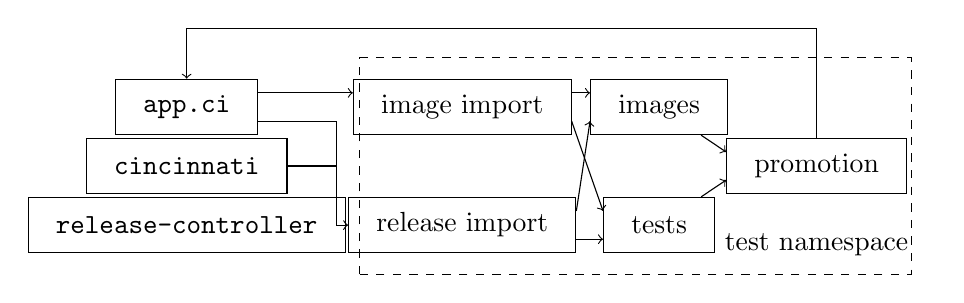
\begin{tikzpicture}[minimum size = 2em, inner xsep = 1em]
        \node[draw] at (4.5, 0) (promotion) {promotion};
        \draw node[draw, minimum width = 4] at (2.5,  0.75) (images) {images};
        \node[draw, minimum width = 4] at (2.5, -0.75) (tests) {tests};
        \node[draw, minimum width = 2]
            at (0, 0.75) (image_import) {image import};
        \node[draw, minimum width = 2]
            at (0, -0.75) (release_import) {release import};
        \node at (-1.6, -0.75) (releases0) {};
        \node[draw] at (-3.5,  0.75) (app_ci) {\texttt{app.ci}};
        \node[draw] at (-3.5, 0) (cincinnati) {\texttt{cincinnati}};
        \node[draw] at (-3.5, -0.75) (rc) {\texttt{release-controller}};
        \node at (4.5, -1) {test namespace};
        \draw[draw, dashed] (-1.3, -1.375) rectangle ++(7, 2.75);
        \draw[->]
            ($ (app_ci.north east)!0.5!(app_ci.east) $)
            -- ($ (image_import.north west)!0.5!(image_import.west) $);
        \draw
            ($ (app_ci.south east)!0.5!(app_ci.east) $)
            -| (releases0.center);
        \draw (cincinnati) -| (releases0.center);
        \draw (rc.east) -| (releases0.center);
        \draw[->] (releases0.center) -- (release_import);
        \draw[->]
            ($ (image_import.north east)!0.5!(image_import.east) $)
            -- ($ (images.north west)!0.5!(images.west) $);
        \draw[->]
            ($ (image_import.south east)!0.5!(image_import.east) $)
            -- ($ (tests.north west)!0.5!(tests.west) $);
        \draw[->]
            ($ (release_import.north east)!0.5!(release_import.east) $)
            -- ($ (images.south west)!0.5!(images.west) $);
        \draw[->]
            ($ (release_import.south east)!0.5!(release_import.east) $)
            -- ($ (tests.south west)!0.5!(tests.west) $);
        \draw[->] (images) -- ($ (promotion.north west)!0.5!(promotion.west) $);
        \draw[->] (tests) -- ($ (promotion.south west)!0.5!(promotion.west) $);
        \draw[->] (promotion) -- ++(0, 1.75) -| (app_ci);
    \end{tikzpicture}
    \note{
        This is the pictorial representation of this process.  Images come from
        the left: base images come from the central registry in \texttt{app.ci}
        (more on that also later), release images come from any of the three
        places, depending on which type of \texttt{releases} field is used.

        The sub-graph which originates in \texttt{app.ci} and returns to it
        finally after the promotion step is the CI cycle.
    }
\end{frame}

\begin{frame}
    \autotitle
    \begin{itemize}
        \item supplemental images
            \begin{itemize}
                \item \url{https://github.com/openshift/release/tree/master/clusters/app.ci/supplemental-ci-images}
                \item \texttt{BuildConfig}s
                \item<2> \texttt{registry.ci.openshift.org/ci/ci-tools-build-root}
            \end{itemize}
        \item image mirroring
            \begin{itemize}
                \item \url{https://github.com/openshift/release/tree/master/core-services/image-mirroring}
                \item Quay/etc. $\leftrightarrow$ \texttt{app.ci}
                \item<2> \texttt{registry.ci.openshift.org/coreos/stream9:9}
            \end{itemize}
        \item ART / OCP builder images
            \begin{itemize}
                \item {\footnotesize\url{https://docs.ci.openshift.org/docs/architecture/images/}}
                \item \url{https://github.com/openshift/ocp-build-data.git}
                \item<2> \texttt{registry.ci.openshift.org/ocp/builder:\ldots}
            \end{itemize}
    \end{itemize}
    \note<1>{
        Base images can come from several places:
        \begin{itemize}
            \item
                Images can be built directly using OpenShift
                \texttt{BuildConfig}s.
            \item
                A mirroring process exists between \texttt{app.ci} and Quay.  It
                is actually bidirectional, but here we are only interested in
                images which are imported from Quay.
            \item
                \textit{Productized} images, used to build official OpenShift
                release images, come from ART.
        \end{itemize}
    }
    \note<2>{
        Note, however, that these images are all located in the \texttt{app.ci}
        central registry.  Initially, they were simply referenced directly, but
        that very soon turned out to not scale to the number of jobs we had at
        the time (which was a small fraction of the current number).
    }
\end{frame}

\subsection{\texttt{dptp-controller-manager}}

\begin{frame}
    \autotitle
    \ttfamily
    \texttt{dptp-controller-manager}
    \begin{itemize}
        \item \href
            {https://github.com/openshift/ci-tools/blob/master/cmd/dptp-controller-manager/}
            {cmd/dptp-controller-manager/}
        \item \href
            {https://github.com/openshift/ci-tools/blob/master/pkg/controller/test-images-distributor/}
            {pkg/controller/test-images-distributor/}
    \end{itemize}
    \note{
        For this reason, there is now a process which imports those images to
        each build cluster whenever required.  It is one of the processes
        executed as part of the \texttt{dptp-controller-manager} (famed cluster
        node assassin) and is named \texttt{test-images-distributor}.
    }
\end{frame}

\begin{frame}[fragile]
    \autotitle
    \small
    \begin{verbatim}
args:
…
- --enable-controller=test_images_distributor
- --enable-controller=promotionreconciler
- --enable-controller=serviceaccount_secret_refresher
- --enable-controller=testimagestreamimportcleaner
…
    \end{verbatim}
    \note{
        The command line shows the enabled controllers, which perform various
        functions in the CI clusters.
    }
\end{frame}

\begin{frame}[fragile]
    \autotitle
    \small
    \begin{verbatim}
…
- --release-repo-git-sync-path=/var/repo/release
- --kubeconfig-dir=/var/kubeconfigs
- --registry-cluster-name=app.ci
- --testImagesDistributorOptions \
    .additional-image-stream-tag=ocp/builder:golang-1.10
…
- --testImagesDistributorOptions \
    .additional-image-stream-tag= \
    ocp/builder:rhel-7-golang-1.11
…
- --testImagesDistributorOptions \
    .additional-image-stream-namespace=ci
- --testImagesDistributorOptions \
    .additional-image-stream=rhcos/machine-os-content
…
    \end{verbatim}
    \note{
        It has a few options to explicitly include image streams and tags\ldots
    }
\end{frame}

\begin{frame}
    \autotitle
    \href
        {https://github.com/openshift/ci-tools/blob/master/pkg/api/helper/imageextraction.go}
        {pkg/api/helper/imageextraction.go}
    \begin{itemize}
        \item \texttt{TestInputImageStreamsFromResolvedConfig}
        \item \texttt{TestInputImageStreamTagsFromResolvedConfig}
    \end{itemize}
    \note{
        \dots{} but its main function is to inspect every \texttt{ci-operator}
        configuration file and extract input images to be synchronized, which it
        does automatically whenever the source streams are changed.
    }
\end{frame}

\subsection{Image promotion}

\begin{frame}[fragile]
    \autotitle
    \small
    \url{https://prow.ci.openshift.org/view/gs/origin-ci-test/logs/branch-ci-openshift-ci-tools-master-images/1561993456950185984}
    \normalsize
    \begin{verbatim}
…
Building src
Build src succeeded after 4m48s
Building bin
Build bin succeeded after 25m54s
Building determinize-peribolos
Building ci-secret-generator
Building ci-operator-config-mirror
…
    \end{verbatim}
    \note{
        Promotion is a relatively simple matter now that we have looked at the
        rest of the pipeline.  We start by building all images not explicitly
        excluded, \ldots
    }
\end{frame}

\begin{frame}[fragile]
    \autotitle
    \begin{verbatim}
…
Build prcreator succeeded after 14m26s
Tagging prcreator into stable
Build private-prow-configs-mirror \
    succeeded after 15m51s
Tagging private-prow-configs-mirror into stable
Promoting tags to ci/${component}:latest: \
    applyconfig, auto-aggregator-job-names, \
    auto-config-brancher, auto-peribolos-sync, \
    auto-sippy-config-generator, …
Ran for 1h7m10s
    \end{verbatim}
    \note{
        \ldots{} then tag them in the \texttt{stable} \texttt{ImageStream} as
        usual, and finally transfer them to the central registry in
        \texttt{app.ci}, where they will be available to future jobs.
    }
\end{frame}

\section{Image pipeline}
\begin{frame}
    \sectiontitleframe
\end{frame}

\begin{frame}[fragile]
    \autotitle
    \scriptsize
    \begin{center}
        \begin{tikzpicture}[
            minimum size = 2em, inner xsep = 1em,
            font = \ttfamily,
            cmd/.style = {font = \ttfamily\tiny},
        ]
            \node[draw] at (0, 0) (root) {root};
            \node[draw, above = of root] (base_images) {\$name};
            \node[draw, right = 1.1 of root] (src) {src};
            \node[draw, above = of src] (bin) {bin};
            \node[draw, right = 1.25 of src] (test_bin) {test-bin};
            \node[draw, above = of test_bin] (rpms) {rpms};
            \node[draw, right = 2 of rpms] (base_rpm_images) {\$name};
            \node[draw, below = of base_rpm_images]
                (base_rpm_images_without) {\$name-without-rpms};
            \node[draw, below = of test_bin] (images) {\$name};
            \node[draw, dashed, below = of base_rpm_images_without]
                (stable) {stable:\$name};
            \node[draw, below = of src] (src_bundle) {src-bundle};
            \node[draw, below = 2.5 of root] (bundles) {\$name};
            \node[draw, below = of src_bundle] (ci_index) {ci-index-*};
            \node[draw, below = of images]
                (ci_index_gen) {ci-index-*-gen};
            \draw[->] (root) -- (src);
            \draw[->] (src) -- (bin);
            \draw[->, dotted] (bin) -- node[cmd, pos = 0.15] {cache} (root);
            \draw[->] (src) -- (test_bin);
            \draw[->] (src) -- (rpms);
            \draw[->] (src) -- (images);
            \draw[->] (bin) -- (rpms);
            \draw[->] (rpms) -- (base_rpm_images);
            \draw[->] (base_rpm_images_without) -- (base_rpm_images);
            \draw[->]
                (src)
                -- node[cmd, pos = 0.3] {}
                (src_bundle);
            \draw[->] (src_bundle) -- (bundles);
            \draw[->, dashed]
                ($ (images.north east)!0.5!(images.east) $) ++(0.9, 0)
                --
                node[cmd, above = 0.25] {.from}
                node[cmd, above] {.inputs}
                ($ (images.north east)!0.5!(images.east) $);
            \draw[->]
                ($ (images.south east)!0.5!(images.east) $)
                -- ($ (stable.south west)!0.5!(stable.west) $);
            \draw[->, dashed] (stable.east) -- ++(0.5, 0);
            \draw[->, dashed]
                (src_bundle.west) ++(-1.75, 0)
                -- node[cmd, above] {.substitutions}
                (src_bundle);
            \draw[->, dashed]
                (ci_index_gen.east) ++(2, 0)
                --
                node[cmd, above = 0.25] {.base\_index}
                node[cmd, above] {.operator\_index}
                (ci_index_gen);
            \draw[->] (ci_index_gen) -- (ci_index);
            \node[cmd, above = 0.25 of root] {build\_root};
            \node[cmd, above = 0 of root] {.use\_build\_cache};
            \node[cmd, above = 0.25 of src] {\$JOB\_SPEC.refs};
            \node[cmd, above = 0 of src] {\$JOB\_SPEC.extra\_refs};
            \node[cmd, above = 0 of bin] {binary\_build\_commands};
            \node[cmd, above = 0 of test_bin] {test\_binary\_build\_commands};
            \node[cmd, above = 0 of rpms] {rpm\_build\_commands};
            \node[cmd, above = 0 of base_rpm_images_without]
                {base\_rpm\_images};
            \node[cmd, above = 0.25 of base_images] {base\_images};
            \node[cmd, above = 0 of base_images] {from\_image};
            \node[cmd, above = 0 of base_rpm_images] {base\_rpm\_images};
            \node[cmd, above = 0 of images] {images};
            \node[cmd, above = 0 of bundles] {operator.bundles};
            \node[cmd, above = 0 of src_bundle] {operator};
            \node[cmd, above = 0 of ci_index] {operator.bundles};
            \node[cmd, above = 0 of ci_index_gen] {operator.bundles};
        \end{tikzpicture}
    \end{center}
    \note{
        Legend:
        \begin{itemize}
            \item
                Solid boxes are pipeline images (tags, technically), solid lines
                are dependencies.
            \item
                The dashed \texttt{stable} box represents the "internal"
                promotion to the stable stream prior to the execution of tests.
            \item
                Dashed lines represent edges not fully depicted since they are
                optional and can be added to any image in the pipeline:
                \begin{itemize}
                    \item
                        Each entry in \texttt{operator.substitutions} makes
                        \texttt{src-bundle} depend on that image.
                    \item
                        The \texttt{operator.substitutions} entry, if specified,
                        makes the \texttt{src-bundle} depend on those images.
                    \item
                        The \texttt{operator.base\_index} entry, if specified,
                        makes all index generator images depend on that image.
                \end{itemize}
        \end{itemize}
    }
\end{frame}


\begin{frame}
    \usebeamertemplate{end page}
\end{frame}

\end{document}
